\documentclass[11pt,a4paper]{article}
\usepackage[utf8]{inputenc}
\usepackage[T1]{fontenc}
\usepackage{amsfonts}
\usepackage{amssymb}
\usepackage{mdframed}
\usepackage{tikz}
\usepackage{tkz-tab}
\usepackage{pgfplots}
\usepackage{xcolor}
\usepackage{fancyhdr}
\usepackage{lastpage}
\usepackage[fleqn]{amsmath}
\setlength{\mathindent}{0pt}

% Spécifications du document
\newcommand{\doctitre}{Les suites} % Ex: Le second degré
\newcommand{\docniveau}{$1^{\text{re}}$ Spécialité mathématiques} % Ex: $1e^{\text{re}}$ Spécialité mathématiques
\newcommand{\doctheme}{Algèbre } % Ex: Algèbre
\newcommand{\doctype}{Démonstrations} % Ex: Démonstrations
\newcommand{\docshorttype}{Démo} % Ex : Démo

% Couleurs pour les graphiques
\definecolor{dark_green}{HTML}{008000}

% Paramètres du document
\RequirePackage{geometry}
\geometry{tmargin=1cm,bmargin=1.9cm,lmargin=1.9cm,rmargin=1.9cm}
\renewcommand{\familydefault}{\sfdefault}
\setlength{\parindent}{0pt}
\title{\doctitre}
\author{\docniveau \\ \doctheme - \doctype}
\date{}
\fancypagestyle{custom}{
  \fancyhf{}
  \renewcommand{\headrulewidth}{0pt}
  \lfoot{\doctheme - \docshorttype}
  \cfoot{\doctitre} % Change \titre to \doctitre
  \rfoot{\thepage/\pageref{LastPage}}
}

% Styles pour les mdframed
\mdfdefinestyle{definitionStyle}{
    leftline=true,
    rightline=false,
    topline=false,
    bottomline=false,
    linewidth=2pt,
    linecolor=black,
    innertopmargin=0pt,
    innerbottommargin=0pt,
    innerrightmargin=0pt,
    innerleftmargin=5pt,
}

\mdfdefinestyle{proprieteStyle}{
    linewidth=1pt,
    linecolor=black,
    innertopmargin=5pt,
    innerbottommargin=5pt,
    innerrightmargin=5pt,
    innerleftmargin=5pt,
}

% ----- DEBUT DU DOCUMENT -----
\begin{document}

% Style et numérotation
\maketitle
\pagestyle{custom}
\thispagestyle{custom}

\section*{II. Suites arithmétiques et géométriques}
\subsection*{1. Suites arithmétiques}

\underline{Démonstrations \emph{(formule explicite)} :}
\begin{equation*}
  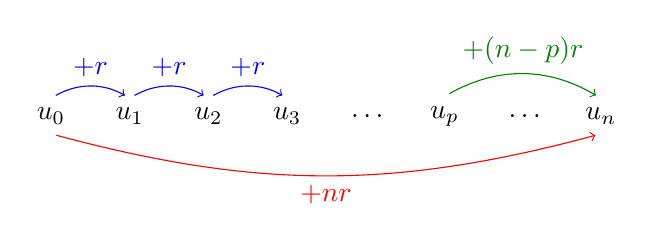
\begin{tikzpicture}[baseline=(math.base)]
    \node[anchor=east] (u0) at (0,0) {$u_0$};
    \node[anchor=east] (u1) at (1,0) {$u_1$};
    \node[anchor=east] (u2) at (2,0) {$u_2$};
    \node[anchor=east] (u3) at (3,0) {$u_3$};
    \node[anchor=east] (d) at (4.1,0) {$\dots$};
    \node[anchor=east] (up) at (5,0) {$u_p$};
    \node[anchor=east] (d) at (6.1,0) {$\dots$};
    \node[anchor=east] (un) at (7,0) {$u_n$};
    \node[inner sep=0] (math) at (u0|-u0.south) {$\phantom{u_0}$};
    \draw[->,blue,shorten >=2pt,shorten <=2pt] (u0.north) to[bend left] node[above,midway] {$+r$} (u1.north);
    \draw[->,blue,shorten >=2pt,shorten <=2pt] (u1.north) to[bend left] node[above,midway] {$+r$} (u2.north);
    \draw[->,blue,shorten >=2pt,shorten <=2pt] (u2.north) to[bend left] node[above,midway] {$+r$} (u3.north);
    \draw[->,dark_green,shorten >=2pt,shorten <=2pt] (up.north) to[bend left] node[above,midway] {$+(n-p)r$} (un.north);
    \draw[->,red,shorten >=2pt,shorten <=2pt] (u0.south) to[bend right=15] node[below,midway] {$+nr$} (un.south);
  \end{tikzpicture}
\end{equation*}

\underline{Démonstrations \emph{(sens de variation)} :}
\begin{equation*}
  \begin{split}
    \text{On calcule }& u_{n+1}-u_n \\
    = \text{ }& u_n+r-u_n \\
    = \text{ }& r
  \end{split}
\end{equation*}
\begin{itemize}
  \item Si $r>0$, $u_{n+1}-u_n>0$ pour tout $n\in\mathbb{N}$. \\
        Donc la suite $u$ est strictement croissante.
  \item Si $r<0$, $u_{n+1}-u_n<0$ pour tout $n\in\mathbb{N}$. \\
        Donc la suite $u$ est strictement décroissante.
  \item Si $r=0$, $u_{n+1}-u_n=0$ pour tout $n\in\mathbb{N}$. \\
        Donc la suite $u$ est constante. \\
\end{itemize}

\underline{Démonstrations \emph{(sommes de termes consécutifs)} :}
\begin{equation*}
  \begin{array}{r c c c c c c c c c c c c c c}
    S=        & 1     & + & 2     & + & 3     & + & \dots & + & (n-2) & + & (n-1) & + & n     \\
    +\quad S= & n     & + & (n-1) & + & (n-2) & + & \dots & + & 3     & + & 2     & + & 1     \\
    \cline{1-14}
    2S=       & (n+1) & + & (n+1) & + & (n+1) & + & \dots & + & (n+1) & + & (n+1) & + & (n+1) \\
  \end{array}
\end{equation*}
\vspace{-12pt}
\begin{equation*}
  \renewcommand{\arraystretch}{2}
  \begin{array}{rrl}
                    & 2S= & n(n+1)                         \\
    \Leftrightarrow & S=  & \displaystyle \frac{n(n+1)}{2}
  \end{array}
\end{equation*}

\newpage

\subsection*{2. Suites géométriques}

\underline{Démonstrations \emph{(formule explicite)} :}
\begin{equation*}
  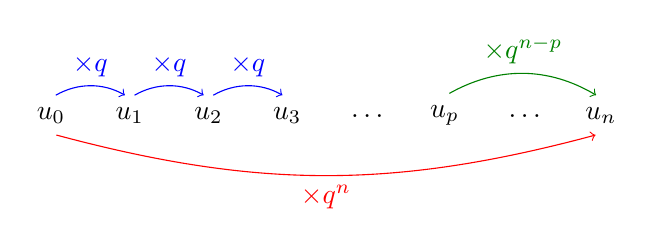
\begin{tikzpicture}[baseline=(math.base)]
    \node[anchor=east] (u0) at (0,0) {$u_0$};
    \node[anchor=east] (u1) at (1,0) {$u_1$};
    \node[anchor=east] (u2) at (2,0) {$u_2$};
    \node[anchor=east] (u3) at (3,0) {$u_3$};
    \node[anchor=east] (d) at (4.1,0) {$\dots$};
    \node[anchor=east] (up) at (5,0) {$u_p$};
    \node[anchor=east] (d) at (6.1,0) {$\dots$};
    \node[anchor=east] (un) at (7,0) {$u_n$};
    \node[inner sep=0] (math) at (u0|-u0.south) {$\phantom{u_0}$};
    \draw[->,blue,shorten >=2pt,shorten <=2pt] (u0.north) to[bend left] node[above,midway] {$\times q$} (u1.north);
    \draw[->,blue,shorten >=2pt,shorten <=2pt] (u1.north) to[bend left] node[above,midway] {$\times q$} (u2.north);
    \draw[->,blue,shorten >=2pt,shorten <=2pt] (u2.north) to[bend left] node[above,midway] {$\times q$} (u3.north);
    \draw[->,dark_green,shorten >=2pt,shorten <=2pt] (up.north) to[bend left] node[above,midway] {$\times q^{n-p}$} (un.north);
    \draw[->,red,shorten >=2pt,shorten <=2pt] (u0.south) to[bend right=15] node[below,midway] {$\times q^n$} (un.south);
  \end{tikzpicture}
\end{equation*}

\underline{Démonstrations \emph{(sens de variation)} :} \\

Comme $u_0>0$, lorsque $q>0$, on a $u_n>0$ pour tout $n\in\mathbb{N}$.
\begin{equation*}
  \begin{split}
    \text{On calcule }& \frac{u_{n+1}}{u_n} \\
    = \text{ }& \frac{q\times u_n}{u_n} \\
    = \text{ }& q
  \end{split}
\end{equation*}

\begin{itemize}
  \item Si $q>1$, on a $\frac{u_{n+1}}{u_n}>1$ et on a $u_{n+1}>u_n$ (car positifs). \\
        Donc la suite $u$ est croissante.
  \item Si $q=1$, on a $u_{n+1}=u_n$ pour tout $n\in\mathbb{N}$. \\
        Donc la suite $u$ est constante.
  \item Si $0<q<1$, on a $0<\frac{u_{n+1}}{u_n}<1$ \\
        Donc $u_{n+1}<u_n$ pour tout $n\in\mathbb{N}$. \\
        Donc la suite $u$ est décroissante.
  \item Lorsque $q<0$, la suite est alternée, c'est à dire que les termes son successivement négatifs et positifs. \\
        Donc la suite n'est ni croissante ni décroissant.
\end{itemize}


\underline{Démonstrations \emph{(sommes de termes consécutifs)} :} \\

On soustrait $S$ à $qS$ et on décale les éléments de $qS$ vers la droite :
\begin{equation*}
  \begin{array}{r c c c c c c c c c c c c c c}
    S=         & 1 & + & q & + & q^2   & + & \dots & +     & q^{n-1} & + & q^n &   &         \\
    -\quad qS= &   &   & q & + & q^2   & + & \dots & \dots & \dots   & + & q^n & + & q^{n+1} \\
    \cline{1-14}
    S-qS=      & 1 & + & 0 & + & \dots & + & \dots & \dots & \dots   & + & 0   & - & q^{n+1} \\
  \end{array}
\end{equation*}
\vspace{-12pt}
\begin{equation*}
  \renewcommand{\arraystretch}{2}
  \begin{array}{ll}
                    & S-qS=    1-q^{n+1}                                                          \\
    \Leftrightarrow & S(1-q)=  1-q^{n+1}                                                          \\
    \Leftrightarrow & \displaystyle S=\frac{1-q^{n+1}}{1-q} \quad\text{($\div1-q$ car $q\not=1$)}
  \end{array}
\end{equation*}

\end{document}